\documentclass{article}
\usepackage{graphicx}
\usepackage[utf8]{inputenc}
\usepackage[italian]{babel}
\usepackage{amsmath}
\usepackage{float}
\usepackage{pdfpages}
\usepackage{multicol}
\usepackage{hyperref}
\usepackage[margin=2.0cm]{geometry}

\title {Viscosimetro a Caduta}
\author{Leonardo Melis, Gianluca Nichetti, Zoya Veronese}
\date{09/04/2025}

\begin{document}

\hrulefill
\begin{flushright}
\textbf{Universit\`a di Padova - Dipartimento Fisica e Astronomia}\\ 
\textbf{Corso:} Sperimentazioni 1 - Canale M-Z.\\
\textbf{Anno accademico:} 2024-25.\\
\textbf{Docenti:} D. Mengoni (\url{daniele.mengoni@unipd.it}) M.~Doro (\url{michele.doro@unipd.it}) \\
\end{flushright}

\bigskip
\noindent

\large{\textbf{Gruppo M3} \\
Leonardo Melis - 2148583 - \url{leonardo.melis@studenti.unipd.it} \\
Gianluca Nichetti - 2137786 - \url{gianluca.nichetti@studenti.unipd.it} \\
Zoya Veronese - 215523 - \url{zoya.veronese@studenti.unipd.it} \\
\begin{verbatim}Data consegna relazione: 09/04/2025\end{verbatim} \hrulefill 

\section*{Viscosimetro a Caduta} }


\begin{multicols}{2}
\setlength{\columnsep}{10mm}

\section{Abstract}
Quest'esperienza con il viscosimetro a caduta ha avuto l'obiettivo di misurare la viscosità di due fluidi, un liquido saponoso e il glicerolo, verificando la validità della legge di Stokes. Lasciando cadere dentro un tubo di plexiglass contenente uno dei due fluidi delle sfere d'acciaio sono state misurate le velocità limite in regime laminare. I dati raccolti sono stati analizzati per calcolare il coefficiente di viscosità e confrontarlo con i valori teorici, considerando le possibili fonti di errore, come effetti di parete, stratificazione della densità e variazioni di temperatura. I risultati hanno confermato la relazione tra viscosità e velocità limite, validando il modello teorico, e hanno evidenziato l'impatto delle sistematiche su tale esperienza.



\section{Introduzione teorica}
La viscosità è una proprietà fondamentale dei fluidi che descrive la loro resistenza al moto relativo tra le particelle costituenti. Nei fluidi newtoniani, la viscosità rimane costante al variare della velocità di taglio, mentre nei fluidi non newtoniani essa può variare in funzione della sollecitazione applicata.
La misura della viscosità può avvenire tramite diverse tecniche, tra cui viscosimetri capillari, rotazionali e a caduta. In particolare, il metodo basato sulla caduta di sfere in un fluido permette di determinare la viscosità sfruttando il moto della sfera. Un modello fondamentale per lo studio della viscosità è la legge di Stokes che descrive la forza di attrito viscoso agente su una sfera in caduta libera attraverso un fluido in regime laminare. Tale forza è proporzionale alla velocità della sfera e alla viscosità del fluido ed è descritta dalla seguente formula:
\begin{equation}
    \vec{F_v}=6\pi r\eta \vec{v}
\end{equation}
nella quale r è raggio, $\eta$ è la viscosità e $\vec{v}$ la velocità. Tale forza si somma alla forza peso:
\begin{equation}
    \vec{F_p}=\frac{4}{3}\pi r^3 \rho \vec{g}
\end{equation}
nella quale r è raggio e $\rho$ è densità della sfera; e alla spinta di Archimede:
\begin{equation} 
    \vec{F_a}=\frac{4}{3}\pi r^3\rho_0 \vec{g}
\end{equation}
nella quale r è raggio e $\rho_0$ la densità. Se $\vec{v}=\vec{v_l}$ velocità limite la risultante delle forze è 0, ciò permette il mantenimento di uno stato di equilibrio. 
\[
\vec{F_v}+\vec{F_p}+\vec{F_a}=0
\]
Date le precedenti formule e considerazioni possiamo ricavare la seguente relazione:
\begin{equation}
    \eta= D^2\frac{\rho- \rho_0}{18 v_l}g
\end{equation}
che esprime la viscosità $\eta$ in funzione delle densità del diametro quadrato $D$ e della velocità limite $v_l$. La condizione di regime laminare è descritta dal numero di Reynolds, rapporto fra la forza di inerzia e la forza di attrito viscoso, che deve rimanere al di sotto di una soglia critica per garantire l'assenza di turbolenze. Il numero di Reynolds si ottiene con la seguente formula:
\[
R=\frac{\rho vD}{\eta}
\]
\
Nella quale $\rho$ è la densità, $v$ la velocità, $D$ il diametro ed $\eta$ la viscosità. Nelle misurazioni effettuate in questa esperienza si sono sempre mantenuti dei parametri tali da poter considerare il regime laminare.
\subsection{Fluidi non Newtoniani}
Nei fluidi non Newtoniani la viscosità non rimane costante ma varia in base a come il fluido viene sollecitato. Esistono diverse tipologie di fluidi non Newtoniani:
\begin{enumerate}
    \item \textbf{Fluidi dilatatori}: se su di essi viene applicata una forza rapida si comportano come un materiale elastico, mentre se sono soggetti a una forza lenta si comportano come dei liquidi. 
    \item \textbf{Fluidi pseudo-plastici}: la loro viscosità diminuisce con l'aumento della velocità di taglio.
    \item \textbf{Fluidi tissotropici}: mostrano una diminuzione della viscosità se su di essi viene applicata una forza di taglio costante, e tornano alla viscosità originaria se lasciati a riposo.
    \item \textbf{Fluidi reologicamente complessi}: hanno le caratteristiche di diversi fluidi non newtoniani.
\end{enumerate}
Il sapone, uno dei fluidi utilizzati nell'esperienza, è un fluido non newtoniano di tipo tissotropico (ciò verrà evidenziato nell'analisi dei dati raccolti).
\subsection{Possibili sistematiche strumentali}
Nello svolgimento dell'esperienza è possibile incorrere in delle sistematiche dovute alla natura del fenomeno e alla struttura dell'apparato:
\begin{enumerate}
    \item \textbf{Effetto fondo e parete}: La legge viene assunta vera per un fluido ideale in un recipiente infinito. Ovviamente nella realtà il recipiente non può essere infinito ma di dimensioni significativamente maggiori rispetto alla sferetta che viene lasciata cadere. Tale effetto causato dall'attrito del fluido con fondo e pareti causa nella raccolta dati una diminuzione della velocità proporzionale al raggio della sferetta; tale sistematica è correggibile mediante la seguente formula:
    \begin{equation}
        v_{\infty}=v_l(1+2.3\frac{r_i}{R})(1+3.3\frac{r_i}{h})
    \end{equation}
    in cui $v_{\infty}$ è la velocità limite che si sarebbe registrata se il recipiente fosse infinito, $v_l$ la velocità limite ricavata, $r_i$ il raggio della sferetta, $R$ il raggio e $h$ l'altezza del recipiente.
    \item \textbf{Temperatura}: Le variazioni di temperatura costituiscono una significativa sistematica per quanto riguarda la misura della viscosità infatti per una variazione di temperatura di 1 C° si dovrebbe registrare una variazione di circa 0.8 poise. Inoltre è stato registrato che la temperatura varia anche con l'aumentare della profondità, infatti la temperatura in cima al recipiente è mediamente 0.5 C° maggiore rispetto che la temperatura sul fondo.
    \item \textbf{Densità media del liquido} Il parametro della densità del liquido $\rho_0$ che compare nella (4) è un valore medio, infatti a causa della pressione la densità sul fondo del recipiente è maggiore e minore in superficie.
    \item \textbf{Densità locale}: Nel liquido con il passaggio delle sferette è possibile che si formino delle bolle d'aria o dei tunnel che vadano a modificare la densità locale. Questo fenomeno non dovrebbe presentarsi in un fluido newtoniano, ma per completezza i test di verifica sono stati effettuati ugualmente (si veda il paragrafo Risultati)
\end{enumerate}
I primi tre fenomeni sono definibili solo per quanto riguarda il glicerolo dato che non siamo a conoscenza della legge che determina l'andamento della viscosità nel liquido saponoso; l'ultimo invece si verifica soprattutto nel liquido non newtoniano.


\section{Metodologia e apparato strumentale}
\subsection{Apparato strumentale e incertezze}
L'apparato sperimentale è composto da un cilindro di plexiglas contenente un liquido, sferette in acciaio (densità $\rho = 7.870 \pm  g/cm^3$) e un cronometro digitale con risoluzione di 0.001 s, quindi con incertezza a priori uniforme pari a 0.0003 s (formula 8 in appendice). Il cilindro (Fig. 1) può contenere un liquido a base di sapone ($\rho = 1.032 \pm 0.001 g/cm^3$) o, in alternativa, glicerolo ($\rho = 1.26 \pm 0.01 g/cm^3$) e presenta traguardi equidistanti di circa 5 cm su un'altezza totale di 50 cm. Con il primo traguardo posto a 7 cm dalla superficie il liquido occupa circa 70 cm in altezza. Le sferette in acciaio hanno diametri compresi tra 1.5 mm e 7.1 mm, con un'incertezza costante di$ \pm0.01 $mm.
\begin{figure}[H] % Posizione dell'immagine (h = here)
    \centering
    
\includegraphics[width=0.15\textwidth]{appstru.jpg}  
    \caption{Struttura apparato strumentale}  
    \label{Fig:1}  
    \end{figure}
    \subsection{Metodologia}
    Le misure sono state effettuate in due giornate distinte per glicerolo e liquido saponoso, applicando la stessa procedura per entrambi i liquidi. Una sferetta di acciaio viene rilasciata mediante il sistema di sgancio del viscosimetro, e un operatore registra manualmente i tempi di percorrenza al raggiungimento dei vari traguardi utilizzando il cronometro. In alcuni casi per le sferette di diametro maggiore le misure sono state raccolte sulla metà dei traguardi (alternati uno si uno no) a causa dell'elevata velocità di caduta delle sferette. Per ogni serie sono state impiegate quattro sferette e calcolate media e deviazione standard (formule 1 e 6 in appendice). Dai tempi misurati è stata determinata la velocità con la seguente formula $v=\Delta s/\Delta t$. Successivamente, è stata calcolata la viscosità (formula (4)) per ogni traguardo e diametro.
    
    Per l'analisi dati sono stati utilizzati diversi test statistici le cui formule specifiche sono interamente riportate in appendice. In particolare è stato svolto il test del $\chi^2$ (con relativi gradi li libertà e p-value); stima dell'indice di Pearson, in alcuni casi anche la sua compatibilità con 1 o 0 (tramite test di Student); e in alcuni grafici anche la compatibilità del coefficiente angolare stimato con 0 (retta orizzontale). 
\section{Risultati}

%istogrammi-----------------------------------------------------------------------------------------------------------------
Dalla raccolta dati è emersa innanzitutto la differenza nelle distribuzioni delle misurazioni nel liquido newtoniano e non.
%istogramma glicerolo--------------------------------------------------------------------------------------------------
\begin{figure}[H] % Posizione dell'immagine (h = here)
    \centering
    

\includegraphics[width=0.5\textwidth]{visco_glicerolo.pdf}  
    \caption{Istogramma rappresentante la distribuzione delle misure di tempo effettuate sul glicerolo (liquido Newtoniano)}  
    \label{Fig:1}  
    \end{figure}
    %istogramma sapone--------------------------------------------------------------------------------------------------
    \begin{figure}[H] % Posizione dell'immagine (h = here)
    \centering 
\includegraphics[width=0.5\textwidth]{visco_sapone.pdf}  
    \caption{Istogramma rappresentante la distribuzione delle misure di tempo effettuate sul sapone (liquido non Newtoniano)} 
    \label{Fig:1}  
    \end{figure}
    %istogramma confronto-------------------------------------------------------------------------------------------------
\begin{figure}[H] % Posizione dell'immagine (h = here)
    \centering
    
\includegraphics[width=0.5\textwidth]{visco_histo.pdf}  
    \caption{Istogramma di confronto tra i due precedenti (Fig. 2 e 3)}  
    \label{Fig:1}  
    \end{figure}
   
    In entrambe le distribuzioni è evidente la differenza tra le misurazioni effettuate con diversi diametri (rappresentate in diverse colorazioni). Misure di tempo maggiori corrispondono a diametri maggiori. Apparentemente le distribuzioni sembrano simili ma osservando l'asse delle ascisse su cui sono riportati i tempi è possibile notare che per il liquido saponoso (Fig.3) la dispersione sull'asse x è maggiore. Ciò è mostrato dalla Fig.4 che pone a confronto i due istogrammi precedenti, il glicerolo (rappresentato in rosso) è concentrato sulla parte sinistra del grafico, mentre il liquido saponoso (blu) è distribuito su tutto il grafico.

    
%legge di stokes---------------------------------------------------------------------------------------------------------
    Per \textbf{verificare la legge di Stokes}, assunte vere la (2) e la (3), abbiamo utilizzato la (4) per verificare la relazione tra viscosità $\eta$, velocità limite e diametri. Per facilitare l'analisi dati, dato che la velocità limite è influenzata dal diametro, è stato scelto di separare lo studio in due parti: la prima è la relazione tra diametri quadrati e il reciproco della velocità e la seconda è la relazione tra i diametri quadrati e la viscosità. La scelta di studiare i diametri quadrati e il reciproco della velocità è dovuta alla natura della legge che con l'utilizzo di tali espressioni è più semplice da rappresentare e interpretare. 
%diametri e velocità glicerolo---------------------------------------------------------------------------------------------
    \begin{figure} % Posizione dell'immagine (h = here)
    \centering
    
\includegraphics[width=0.5\textwidth]{gli1.1 nocorrezione.pdf}  
    \caption{Questo grafico mostra la relazione tra diametri quadrati e reciproci delle velocità nel glicerolo}  
    \label{Fig:1}  
    \end{figure}
\begin{table}
\centering
%\renewcommand{\arraystretch}{1.3}
\begin{tabular}{|p{3.5cm}|p{3.5cm}|}
\hline
\small
\textbf{Parametro} & \textbf{Valore} \\ \hline
\textbf{Parametri interpolazione} &$y=(2485\pm13)x+(0.00003\pm0.00004)$ \\ \hline
\textbf{Indice di Pearson} & 0.99$\pm$0.01 \\ \hline
compatibilità indice con 1(p-value) & 0.99\\ \hline
t indice & 0.013\\ \hline
gradi di libertà indice  & 3\\ \hline
\textbf{$\chi^2$ misurato} &  4.87\\ \hline 
gradi di libertà&  3\\ \hline
p-value&  0.18\\ \hline
\end{tabular}
\caption{Dati analisi grafico Fig.5 }
\end{table}
 
%diametri e eta glicerolo----------------------------------------------------------------------------------------------------
    \begin{figure}[H] % Posizione dell'immagine (h = here)
    \centering
    
\includegraphics[width=0.5\textwidth]{gli1.2 nocorrezione.pdf}  
    \caption{Questo grafico mostra la relazione tra diametri quadrati e viscosità nel glicerolo}  
    \label{Fig:1}  
    \end{figure}
    \begin{table}[h!]
\centering
\begin{tabular}{|p{3.5cm}|p{3.5cm}|}
\hline
\small
\textbf{Parametro} & \textbf{Valore} \\ \hline
\textbf{Parametri interpolazione} & $y=(1130\pm920)x+(1.44\pm 0.01)$ \\ \hline
\textbf{Indice di Pearson} & 0.9$\pm$0.2 \\ \hline
\textbf{$\chi^2$ misurato} &  0.55\\ \hline 
gradi di libertà&  3\\ \hline
p-value&  0.91\\ \hline
compatibilità con pendenza nulla (p-value, 2 code)& 2$\times10^{-20}$ \\ \hline
\end{tabular}
\caption{Dati analisi grafico Fig.6 }
\end{table}


   Per quanto riguarda \textbf{il glicerolo} è possibile osservare nel grafico (Fig.5) come la linearità tra velocità e diametri quadrati sia ipotesi plausibile, si veda valore del $\chi^2$ e p-value in tabella 1; anche l'indice di Pearson conferma tale ipotesi. Per quanto riguarda il secondo grafico (Fig.6) il risultato teorico dovrebbe essere una linea orizzontale in quanto $\eta$ in un fluido newtoniano dovrebbe risultare costante. Dai valori di p-value, $\chi^2$ e indice di Pearson (si veda tabella 2) non possiamo accettare tale ipotesi anche se le incertezze sono molto grandi. Per verificare se tale discrepanza è dovuta alla sistematica fondo parete è stata applicata la correzione (5) con applicata anche la relativa propagazione delle incertezze (formula 10 in appendice) e ne è stata fatta nuovamente l'analisi.
%diametri e velocità glicerolo corretto--------------------------------------------------------------------------------------
   \begin{figure}[H]% Posizione dell'immagine (h = here)
    \centering
    
\includegraphics[width=0.5\textwidth]{gli1.1.pdf} 
    \caption{Questo grafico mostra la relazione tra diametri quadrati e reciproci delle velocità nel glicerolo con applicata la correzione fondo-parete}  
    \label{Fig:1}  
    \end{figure}
\begin{table}[H]
\centering
\begin{tabular}{|p{3.5cm}|p{3.5cm}|}
\hline
\small
\textbf{Parametro} & \textbf{Valore} \\ \hline
\textbf{Parametri interpolazione} & $y=(2724\pm14)x+(-0.00029\pm 0.00004)$\\ \hline
\textbf{Indice di Pearson} & 0.99$\pm$0.01 \\ \hline
compatibilità indice con 1(p-value) & 0.99\\ \hline
t indice & 0.009\\ \hline
gradi di libertà indice  & 3\\ \hline
\textbf{$\chi^2$ misurato} &  9.07\\ \hline 
gradi di libertà&  3\\ \hline
p-value&  0.03\\ \hline
\end{tabular}
\caption{Dati analisi grafico Fig.7 }
\end{table}
%diametri eta glicerolo corretti-------------------------------------------------------------------------------------------------
    \begin{figure}[h] % Posizione dell'immagine (h = here)
    \centering
    
\includegraphics[width=0.5\textwidth]{gli1.2.pdf} 
    \caption{Questo grafico mostra la relazione tra diametri quadrati e viscosità nel glicerolo con correzione fondo-parete}  
    \label{Fig:1}  
    \end{figure}
    \begin{table}[h]
\centering
\begin{tabular}{|p{3.5cm}|p{3.5cm}|}
\hline
\small
\textbf{Parametro} & \textbf{Valore} \\ \hline
\textbf{Parametri interpolazione} & $y=(-3470\pm810)x+(1.28\pm 0.01)$\\ \hline
\textbf{Indice di Pearson} & -0.9$\pm$0.2 \\ \hline
\textbf{$\chi^2$ misurato} &  2.24\\ \hline 
gradi di libertà&  3\\ \hline
p-value&  0.5\\ \hline
compatibilità con pendenza nulla (p-value, 2 code)& 0.01 \\ \hline
\end{tabular}
\caption{Dati analisi grafico Fig.8 }
\end{table}
Il grafico velocità-diametri (Fig.7) con correzione presenta un $\chi^2$ leggermente peggiore, che non è particolarmente rilevante per la valutazione effettuata (in quanto non stiamo valutando l'interpolazione), e una compatibilità migliore dell'indice di Pearson. 
Sul grafico viscosità-diametri invece si notano significativi cambiamenti: l'andamento risulta completamente opposto, i valori di $\eta$ relativi a diametri maggiori sono stati ridotti di più rispetto agli altri, dato che la correzione è proporzionale al raggio della sferetta, e a differenza dell'andamento descritto precedentemente,  questo può essere ricondotto ad un ulteriore sistematica ovvero la variazione della temperatura che verrà discussa nel paragrafo successivo ("Discussione di ulteriori sistematiche").

Per quanto riguarda \textbf{il liquido saponoso} invece dati i grafici velocità-diametri (Fig.8) e viscosità-diametri (Fig.9) si nota come i dati siano quasi del tutto in disaccordo con le relazioni verificate nel glicerolo. Quest'affermazione è supportata dai valori risultanti dal test del $\chi^2$ riportati nelle tabelle.
%sapone velocità diametri no correzione----------------------------------------------------------------------------------------

 \begin{figure}[h]% Posizione dell'immagine (h = here)
    \centering
    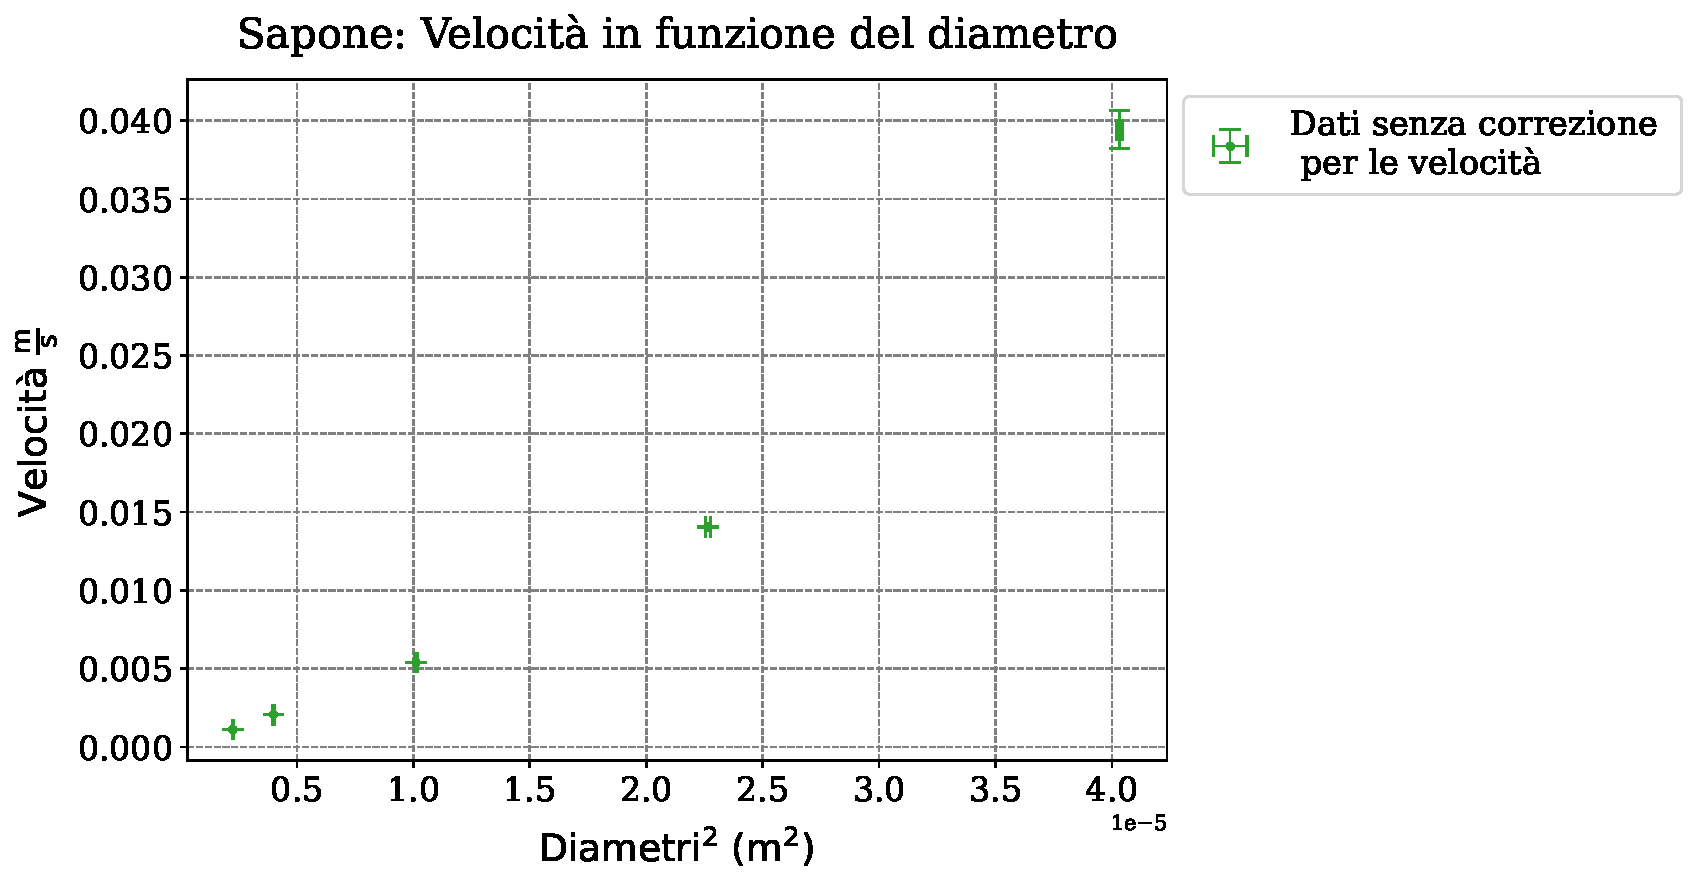
\includegraphics[width=0.5\textwidth]{sap1.1 nocorrezione.pdf} 
    \caption{Questo grafico mostra la relazione tra diametri quadrati e velocità nel sapone}  
    \label{Fig:1}  
    \end{figure}
\begin{table}[h!]
\centering
\begin{tabular}{|p{3.5cm}|p{3.5cm}|}
\hline
\small
\textbf{Parametro} & \textbf{Valore} \\ \hline
\textbf{Parametri interpolazione} & $y=(603\pm2)x+(-0.00033\pm 0.00001)$\\ \hline
\textbf{Indice di Pearson} & 0.98$\pm$0.12 \\ \hline
\textbf{$\chi^2$ misurato} &  637\\ \hline 
gradi di libertà&  3\\ \hline
p-value&  9.23\\ \hline
\end{tabular}
\caption{Dati analisi grafico Fig.9 }
\end{table}
%sapone eta diametri no correzione-----------------------------------------------------------------------------------------------------------------------------------------------------
    \begin{figure}[h] % Posizione dell'immagine (h = here)
    \centering
    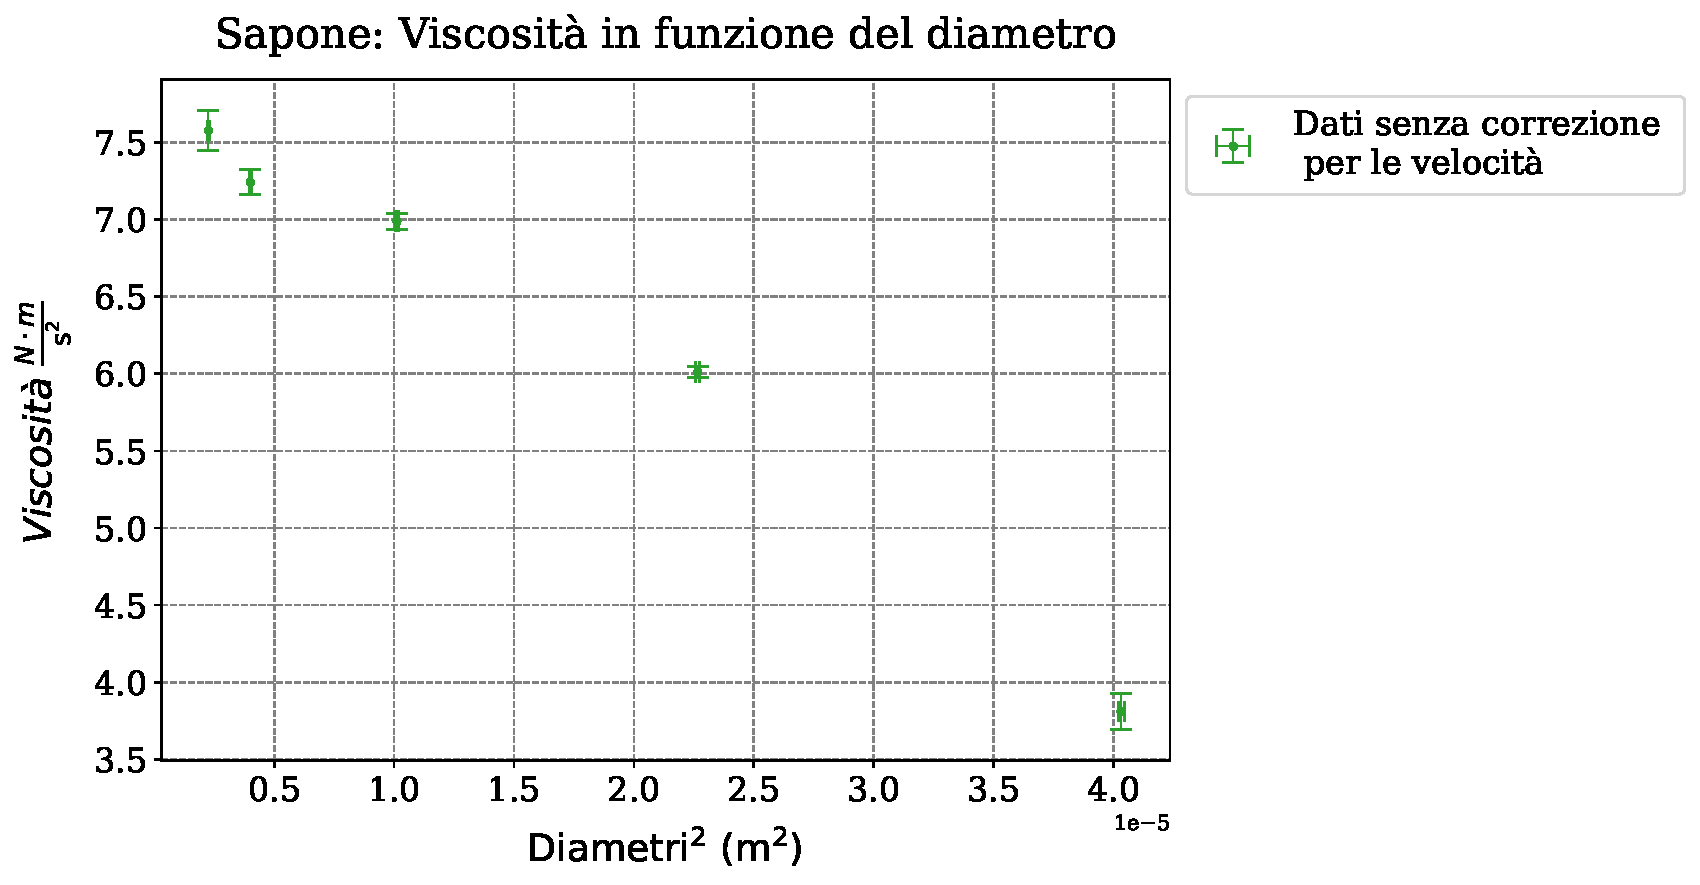
\includegraphics[width=0.5\textwidth]{sap1.2 nocorrezione.pdf} 
    \caption{Questo grafico mostra la relazione tra diametri quadrati e viscosità nel sapone}  
    \label{Fig:1}  
    \end{figure}
    \begin{table} [h]
\centering
\begin{tabular}{|p{3.5cm}|p{3.5cm}|}
\hline
\small
\textbf{Parametro} & \textbf{Valore} \\ \hline
\textbf{Parametri interpolazione} & $y=(-84900\pm2800)x+(7.84\pm 0.06)$\\ \hline
\textbf{Indice di Pearson} & -0.99$\pm$0.08 \\ \hline
\textbf{$\chi^2$ misurato} &  44.3\\ \hline 
gradi di libertà&  3\\ \hline
p-value&  1.3\\ \hline
compatibilità con pendenza nulla (p-value, 2 code)& 7.9 \\ \hline
\end{tabular}
\caption{Dati analisi grafico Fig.10 }
\end{table}

In particolare già dato l'andamento decrescente del grafico (Fig.9) applicare una correzione di fondo-parete non sarebbe proficuo, anzi renderebbe le stime di viscosità ancora più distanti fra loro. In ogni caso il sapone è un liquido non Newtoniano quindi i dati raccolti sono coerenti con le ipotesi teoriche.

%verifica di vl ------------------------------------------------------------------------------------------------------------------------------------------------------------------------

Per poter trarre le precedenti considerazioni però è necessario verificare che la velocità raggiunta $v_l$ sia effettivamente la velocità limite quindi che il corpo non acceleri durante la caduta. Questo è possibile verificando la relazione lineare fra tempi e spazi percorsi. Dato il riscontro positivo della correzione fondo-parete è stato deciso di effettuare il test sui dati già corretti.

Dagli ottimi valori di $\chi^2$ e indice di Pearson (Tab.7 e 8) è possibile affermare che l'andamento è perfettamente lineare, quindi la velocità misurata è effettivamente quella limite per entrambi i fluidi.

\begin{figure}[H]
    \centering
    
\includegraphics[width=0.50\textwidth]{gli2.pdf} 
    \caption{Questo grafico mostra la relazione tra spazi e tempi durante la discesa del corpo nel glicerolo a ciascun traguardo, i diversi diametri sono indicati in diverse colorazioni.}  
    \label{Fig:1}  
    \end{figure}
    
    %\vspace*{2cm}
    
\begin{table}[H]
\centering
\small
%\renewcommand{\arraystretch}{1.3}
\begin{tabular}{|p{2cm}|p{3cm}|p{2cm}|}
\hline
\textbf{Serie} & \textbf{Parametro} & \textbf{Valore} \\ \hline
diametro 1.5mm & Parametri interpolazione & $y=(178.2\pm 0.5)x + (-0.25\pm 0.08) $ \\ \hline
 & Indice di Pearson & $0.999 \pm 0.002$ \\ \hline
 & $\chi^2$ misurato & 1.97 \\ \hline 
 & Gradi di libertà & 8 \\ \hline
 & p-value & 0.98 \\ \hline
diametro 2.0mm & Parametri interpolazione & $y=(99.9\pm 0.3)x + (-0.24\pm 0.04) $ \\ \hline
& Indice di Pearson & 0.999$\pm$0.007 \\ \hline
&$\chi^2$ misurato &  8.77\\ \hline 
&gradi di libertà&  8\\ \hline
&p-value&  0.36\\ \hline
diametro 3.2mm & Parametri interpolazione & $y=(40.0\pm 0.2)x + (-0.12\pm 0.04) $ \\ \hline 
& Indice di Pearson & 0.999$\pm$0.004 \\ \hline
&$\chi^2$ misurato &  4.13\\ \hline 
&gradi di libertà&  8\\ \hline
&p-value&  0.84\\ \hline
diametro 4.8mm & Parametri interpolazione & $y=(17.8\pm 0.3)x + (-0.02\pm 0.08) $ \\ \hline 
& Indice di Pearson & 0.999$\pm$0.004 \\ \hline
&$\chi^2$ misurato &  0.19\\ \hline 
&gradi di libertà&  3\\ \hline
&p-value&  0.98\\ \hline
diametro 6.4mm & Parametri interpolazione & $y=(10.3\pm 0.2)x + (0.07\pm 0.06) $ \\ \hline
& Indice di Pearson & 0.999$\pm$0.005 \\ \hline
&$\chi^2$ misurato &  0.19\\ \hline 
&gradi di libertà&  3\\ \hline
&p-value&  0.98\\ \hline
\end{tabular}
\caption{Dati analisi grafico Fig.11 }
\end{table}


\begin{figure} [H]
    \centering
    
\includegraphics[width=0.50\textwidth]{sap2.pdf} 
    \caption{Questo grafico mostra la relazione tra spazi e tempi durante la discesa del corpo nel sapone a ciascun traguardo, i diversi diametri sono indicati in diverse colorazioni.}  
    \label{Fig:1}  
    \end{figure}

    
\begin{table} [H]
\centering
\small
\begin{tabular}{|p{2cm}|p{3cm}|p{2cm}|}
\hline
\textbf{Serie} & \textbf{Parametro} & \textbf{Valore} \\ \hline
diametro 1.5mm & Parametri interpolazione & $y=(904\pm 9)x + (-0.6\pm 1.3) $ \\ \hline
& Indice di Pearson & 1.0000$\pm$0.0003 \\ \hline
&$\chi^2$ misurato &  0.003\\ \hline 
&gradi di libertà&  8\\ \hline
&p-value&  0.99\\ \hline
diametro 2.0mm& Parametri interpolazione & $y=(486\pm 3)x + (-0.5\pm 0.3) $ \\ \hline
& Indice di Pearson & 1.0000$\pm$0.0007 \\ \hline
&$\chi^2$ misurato &  0.006\\ \hline 
&gradi di libertà&  8\\ \hline
&p-value&  0.99\\ \hline
diametro 3.2mm & Parametri interpolazione & $y=(185.5\pm 0.8)x + (-0.7\pm 0.3) $ \\ \hline
& Indice di Pearson & 0.99$\pm$0.01 \\ \hline
&$\chi^2$ misurato &  0.81\\ \hline 
&gradi di libertà&  8\\ \hline
&p-value&  0.99\\ \hline
diametro 4.8mm & Parametri interpolazione & $y=(71.2\pm 0.3)x + (-0.26\pm 0.08) $ \\ \hline
& Indice di Pearson & 0.999$\pm$0.002 \\ \hline
&$\chi^2$ misurato &  1.63\\ \hline 
&gradi di libertà&  8\\ \hline
&p-value&  0.99\\ \hline
diametro 6.4mm & Parametri interpolazione & $y=(25.4\pm 0.7)x + (-0.8\pm 0.2) $ \\ \hline
& Indice di Pearson & 0.99$\pm$0.01 \\ \hline
&$\chi^2$ misurato &  0.29\\ \hline 
&gradi di libertà&  4\\ \hline
&p-value&  0.96\\ \hline
\end{tabular}
\caption{Dati analisi grafico Fig.12 }
\end{table}
%\vspace*{5cm}

%sostituire grafici (Leo)

\section{Discussione dei risultati}
%compatibilità misure glicerolo--------------------------------------------------------------------------------------------------------------------------------------------
\subsection{Compatibilità delle misure}
Dall'introduzione teorica è noto che la viscosità per i liquidi newtoniani dovrebbe essere costante, perciò le misure raccolte per ciascuna sferetta per ciascun traguardo dovrebbero poi ricondurre a misure di viscosità compatibili fra loro. Fenomeno invece che non dovrebbe essere registrato nel liquido saponoso.   
\begin{figure}[H] % Posizione dell'immagine (h = here)
    \centering
    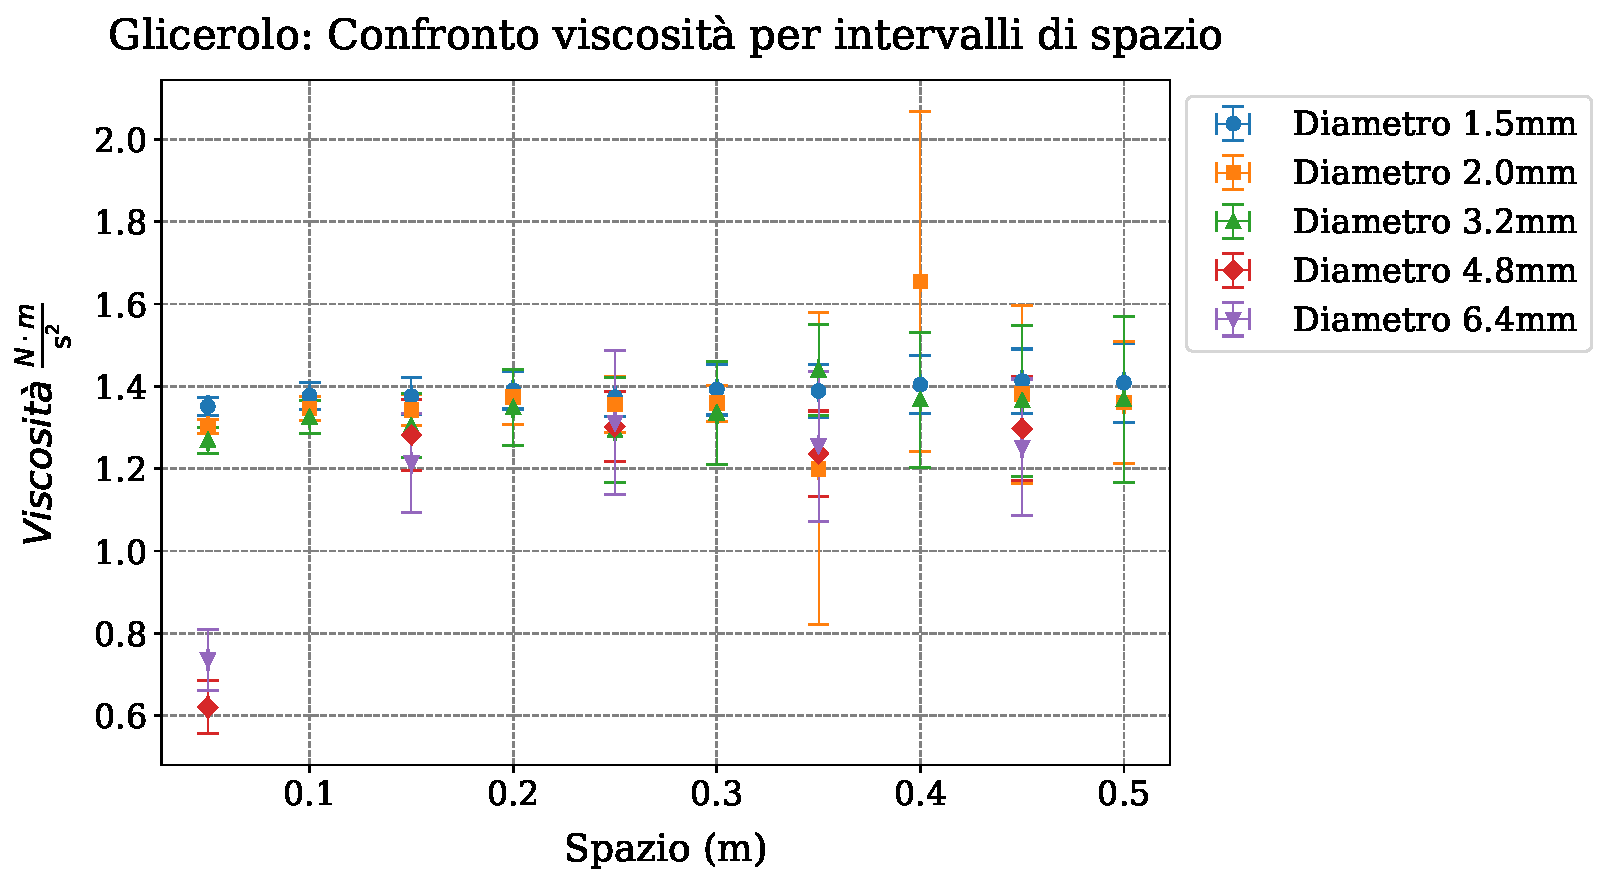
\includegraphics[width=0.5\textwidth]{gli4.1.pdf}  
    \caption{Questo grafico rappresenta i vari valori di viscosità ricavati per ciascun diametro per ciascun traguardo dell'apparato strumentale con glicerolo. Fare riferimento alla legenda della Fig.14.}  
    \label{Fig:1}  
    \end{figure}
    \begin{figure}[H]
    \centering
    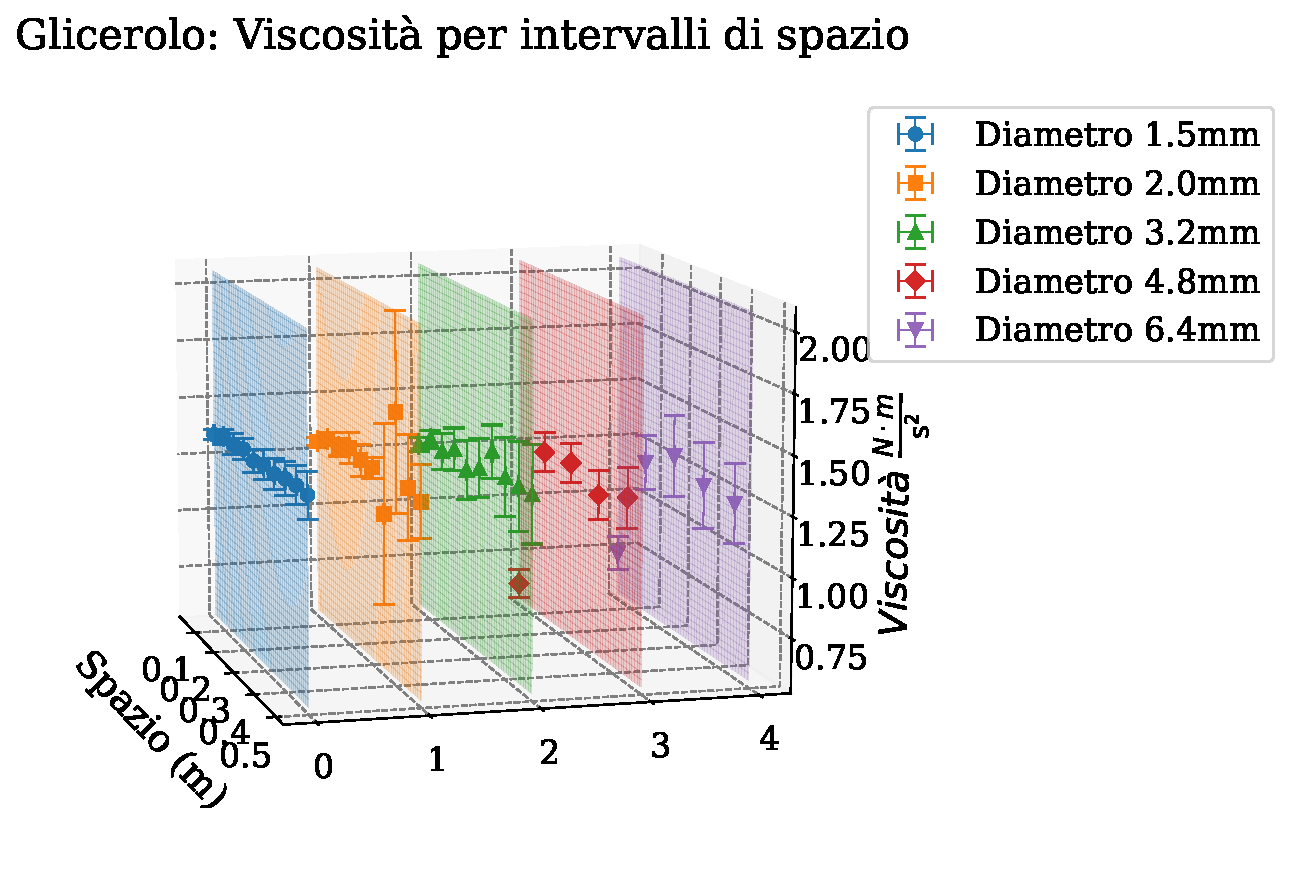
\includegraphics[width=0.52\textwidth]{gli4.2.pdf}  
    \caption{Questo grafico rappresenta la Fig.13 vista in 3 dimensioni, per poter apprezzare meglio la distinzione fra i vari diametri.}  
    \label{Fig:1}  
    \end{figure}
\begin{table}[H]
\centering
%\renewcommand{\arraystretch}{1.3}
\begin{tabular}{|p{1cm}|p{4.5cm}|p{1cm}|}
\hline
\small
\textbf{Serie} & \textbf{Valori interpolazione} & \textbf{p-value} \\ \hline
1 & $y = (0.1 \pm 0.1)x + (1.35 \pm 0.02)$ & 0.25 \\ \hline
2 & $y = (0.2 \pm 0.1)x + (1.30 \pm 0.01)$ & 0.12 \\ \hline
3 & $y = (0.3 \pm 0.2)x + (1.27 \pm 0.03)$ & 0.16 \\ \hline
4 & $y = (1.8 \pm 0.2)x + (0.69 \pm 0.06)$ & 0.003 \\ \hline
5 & $y = (1.5 \pm 0.4)x + (0.74 \pm 0.08)$ & 0.02 \\ \hline
\end{tabular}
\caption{Dati analisi grafico Fig.13 e 14. Per compattezza si riportano solo i parametri di interpolazione e il p-value derivante dal test di compatibilità con una retta orizzontale. I risultati completi sono riportati in appendice.}
\end{table}

 Osservando i grafici si nota che l'andamento generale è costante, fatta eccezione per qualche misura che risulta non compatibile con le altre. La retta che meglio descrive l'andamento dei dati per ciascuna delle prime tre serie, sebbene talvolta con un errore relativo (formula 11 in appendice) del 100\% , sono compatibili con una retta orizzontale. Le uniche interpolazioni di poco incompatibili sono le ultime, fatto probabilmente dovuto all'elevata velocità limite delle sferette di diametro massimo che ha intaccato la precisione della misura più che nelle altre serie.
%incompatibilità misure sapone---------------------------------------------------------------------------------------------------------------------------------------------------
 \begin{figure}[H] % Posizione dell'immagine (h = here)
    \centering
    
\includegraphics[width=0.5\textwidth]{sap4.1.pdf}  
    \caption{Questo grafico rappresenta i vari valori di viscosità ricavati per ciascun diametro per ciascun traguardo dell'apparato strumentale con liquido saponoso. Fare riferimento alla legenda della Fig.16.}  
    \label{Fig:1}  
    \end{figure}
\begin{figure}[H] % Posizione dell'immagine (h = here)
    \centering
    
\includegraphics[width=0.52\textwidth]{sap4.2.pdf}  
    \caption{Questo grafico rappresenta la Fig.15 vista in 3 dimensioni, per poter apprezzare meglio la distinzione fra i vari diametri.}  
    \label{Fig:1}  
    \end{figure}
\begin{table}[H]
\centering
\renewcommand{\arraystretch}{1.3}
\begin{tabular}{|p{1cm}|p{4.5cm}|p{1cm}|}
\hline
\small
\textbf{Serie} & \textbf{Valori interpolazione} & \textbf{p-value} \\ \hline
1 & $y = (0 \pm 2)x + (7.5 \pm 0.3)$ & 0.85 \\ \hline
2 & $y = (0 \pm 1)x + (7.1 \pm 0.1)$ & 0.55 \\ \hline
3 & $y = (0.6 \pm 0.8)x + (6.7 \pm 0.3)$ & 0.49\\ \hline
4 & $y = (0.6 \pm 0.6)x + (5.8 \pm 0.2)$ & 0.99\\ \hline
5 & $y = (4 \pm 1)x + (2.5 \pm 0.3)$ & 0.05 \\ \hline
\end{tabular}
\caption{Dati analisi grafico Fig.~13 e 14. Per compattezza si riportano solo i parametri di interpolazione e il p-value derivante dal test di compatibilità con una retta orizzontale. I risultati completi sono riportati in appendice.}
\end{table}

Anche in questo set di dati, nonostante riguardi un liquido non newtoniano, i dati delle interpolazioni sono quasi tutti compatibili con quelli di una retta orizzontale (tranne per l'ultima serie che ha coefficiente angolare 4). È comunque bene evidenziare le incertezze di tali stime che sono sempre superiori o uguali ad un errore relativo del 100\% (formula 11 in appendice). Ciò evidenzia una maggiore oscillazione delle misure rispetto al liquido non newtoniano che comporta maggiori incertezze; quindi, nonostante venga mantenuto l'andamento lineare, le misure del liquido saponoso risultano compatibili ma con incertezze molto grandi.
\subsection{Discussione di ulteriori sistematiche}
%aumento eta con la profondità--------------------------------------------------------------------------------------------------
Un altro effetto sistematico che potrebbe essersi presentato sul glicerolo è un progressivo aumento della viscosità $\eta$ mano a mano che la sfera procede nella sua caduta. Per valutare la presenza di tale sistematica si è potuto utilizzare i grafici già precedentemente esposti (Fig.13 e 14). Infatti le conseguenze di questa sistematica sui dati sarebbero delle rette interpolanti a coefficiente angolare negativo ma , come si può notare dai dati nella tabella 9, nessuna delle rette presenta un coefficiente negativo, nemmeno la quinta serie. Quindi è possibile affermare che tale sistematica non ha avuto un incidenza significativa sui dati raccolti.

%stima temperatura--------------------------------------------------------------------------------------------------------------------
Riprendendo il grafico Fig.8 era già stato anticipato che il suo andamento decrescente è spiegato da una variazione di temperatura: nella stanza, durante le misurazioni, è stato registrato un aumento della temperatura di circa 2° (da 20° a 22°), con l'ausilio di un calcolatore online*, è stato verificato se tale escursione termica potesse essere compatibile con la variazione nel tempo della viscosità tenendo conto di due aspetti: 
\begin{enumerate}
    \item Le misure sono state prese a partire dalle sferette con raggio inferiore proseguendo poi in ordine crescente 
    \item La temperatura, internamente al liquido, non ha la stessa variazione della stanza ma una variazione di circa la metà, quindi 1°.
\end{enumerate}
\renewcommand{\thefootnote}{\fnsymbol{footnote}}
\footnotetext[1]{Link al calcolatore:\\ \url{https://www.met.reading.ac.uk/~sws04cdw/viscosity_calc.html}}
\renewcommand{\thefootnote}{\arabic{footnote}}
Il risultato, considerando una miscela di glicerolo al $99.9\%$ e acqua (combinazione più probabile basandosi sui dati raccolti), coincide con un aumento della temperatura di 0.9° da 20.15° a 21.05°; soluzione compatibile con l'ipotesi precedentemente fornita. La trattazione di questa sistematica è stata svolta in maniera approssimativa in quanto non è stato possibile effettuare delle misurazioni più precise e stimarne un'incertezza, per questo è stato deciso di non apportare nessuna correzione ai dati.

%effetto memoria------------------------------------------------------------------------------------------------------------------------
L'ultima sistematica che rimane da verificare è l'effetto memoria che ci si aspetta di registrare nel liquido saponoso e non nel glicerolo. In ausilio possiamo utilizzare i seguenti grafici: Fig.17 e 18.
\begin{figure}[H] % Posizione dell'immagine (h = here)
    \centering
    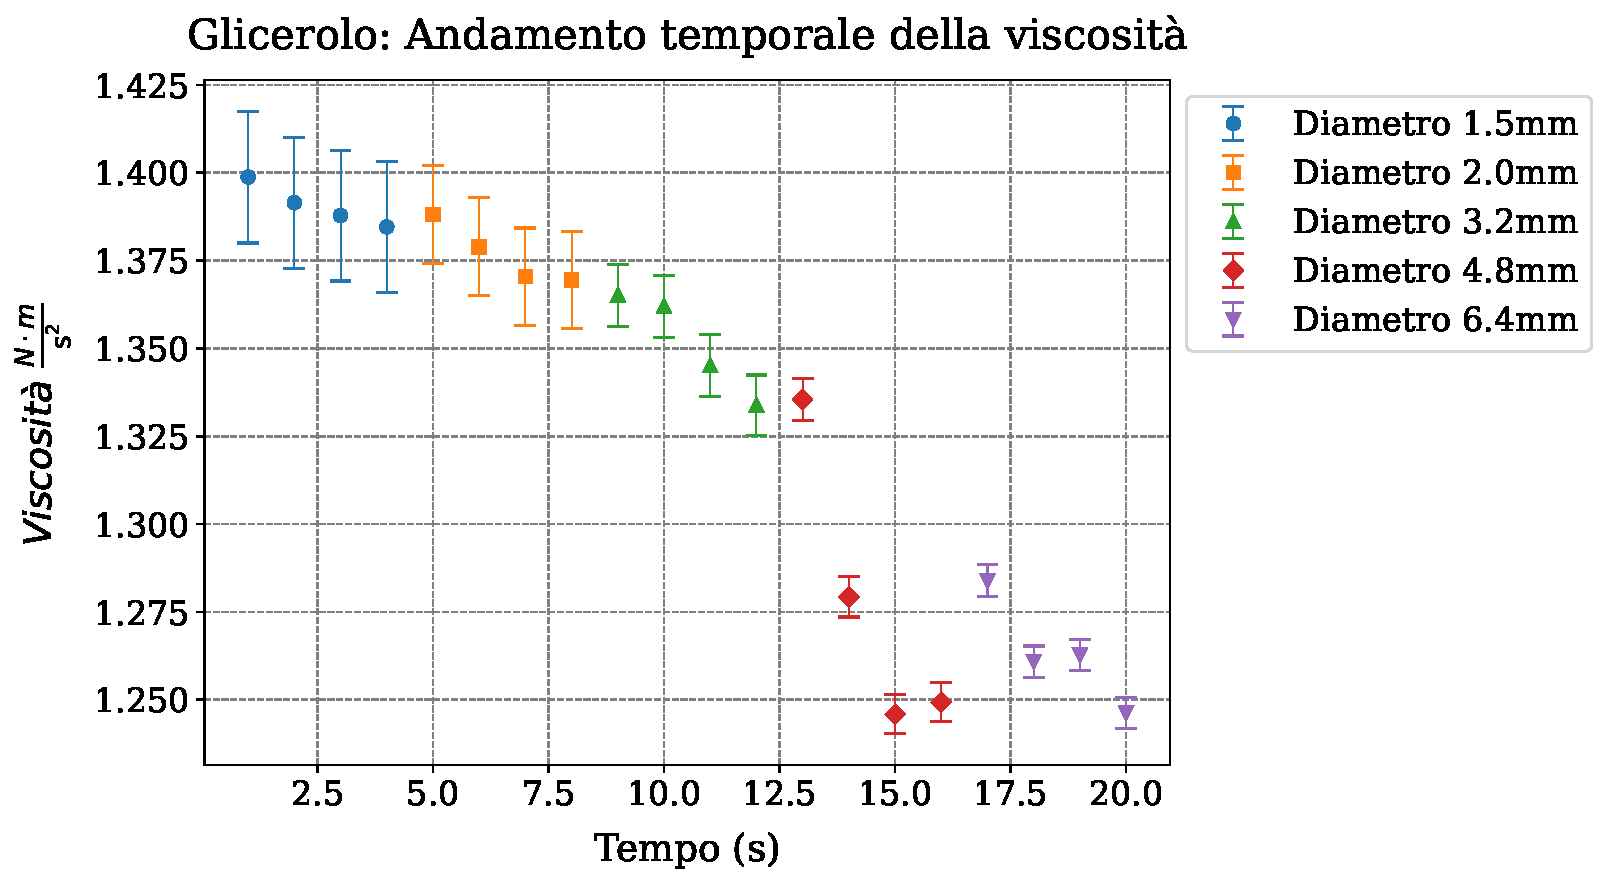
\includegraphics[width=0.52\textwidth]{gli5.pdf}  
    \caption{Questo grafico rappresenta le medie di tutte le n-esime misurazioni (da 1 a 4) fatte con le palline dello stesso diametro in successione temporale nel glicerolo, in modo tale da verificare se per ogni diametro ci sia una variazione dalla prima misura all'ultima.}  
    \label{Fig:1}  
    \end{figure}
\begin{table}[H]
\centering
\small

\begin{tabular}{|p{1cm}|p{4.5cm}|p{1cm}|}
\hline
\textbf{Serie} & \textbf{Valori interpolazione} & \textbf{p-value} \\ \hline
1 & $y = (-0.004 \pm 0.008)x + (1.40 \pm 0.02)$ & 0.85 \\ \hline
2 & $y = (-0.006 \pm 0.006)x + (1.42 \pm 0.04)$ & 0.38 \\ \hline
3 & $y = (-0.011 \pm 0.004)x + (1.47 \pm 0.04)$ & 0.07\\ \hline
4 & $y = (-0.029\pm 0.002)x + (1.69 \pm 0.04)$ & 0.002\\ \hline
5 & $y = (-0.011 \pm 0.002)x + (1.47 \pm 0.04)$ & 0.01 \\ \hline
\end{tabular}
\caption{Dati analisi grafico Fig.17. Per compattezza si riportano solo i parametri di interpolazione e il p-value derivante dal test di compatibilità con una retta orizzontale. I risultati completi sono riportati in appendice.}
\end{table}

\begin{figure}[H] % Posizione dell'immagine (h = here)
    \centering
    
\includegraphics[width=0.52\textwidth]{sap5.pdf}  
    \caption{Questo grafico rappresenta le medie di tutte le n-esime misurazioni (da 1 a 4) fatte con le palline dello stesso diametro in successione temporale nel liquido saponoso, in modo tale da verificare se per ogni diametro ci sia una variazione dalla prima misura all'ultima.}  
    \label{Fig:1}  
    \end{figure}
\begin{table}[H]
\centering

\begin{tabular}{|p{1cm}|p{4.5cm}|p{1cm}|}
\hline
\small
\textbf{Serie} & \textbf{Valori interpolazione} & \textbf{p-value} \\ \hline
1 & $y = (-0.12 \pm 0.04)x + (7.87 \pm 0.12)$ & 0.08 \\ \hline
2 & $y = (-0.06 \pm 0.03)x + (7.67 \pm 0.21)$ & 0.14 \\ \hline
3 & $y = (0.01 \pm 0.01)x + (6.91 \pm 0.21)$ & 0.63\\ \hline
4 & $y = (-0.02\pm 0.01)x + (6.35 \pm 0.16)$ & 0.12\\ \hline
5 & $y = (-0.05 \pm 0.005)x + (4.90 \pm 0.10)$ & 0.001 \\ \hline
\end{tabular}
\caption{Dati analisi grafico Fig.18. Per compattezza si riportano solo i parametri di interpolazione e il p-value derivante dal test di compatibilità con una retta orizzontale. I risultati completi sono riportati in appendice.}
\end{table}
 Escludendo le ultime due serie delle misure sul glicerolo, che probabilmente a causa dell'elevata velocità di discesa hanno riportato valori meno precisi, possiamo vedere che in realtà l'effetto memoria è visibile su entrambi i fluidi e che i valori sono approssimativamente gli stessi. Infatti interpolando ciascuna serie con una retta indipendente notiamo che i coefficienti sono negativi, anche se si discostano molto poco dallo 0; e nella maggior parte dei casi hanno una buona compatibilità con una retta orizzontale. Quindi è possibile affermare che l'effetto memoria è presente ma minimo su entrambi i fluidi.   

\section{Conclusione}
\begin{figure}[H]
    \centering
    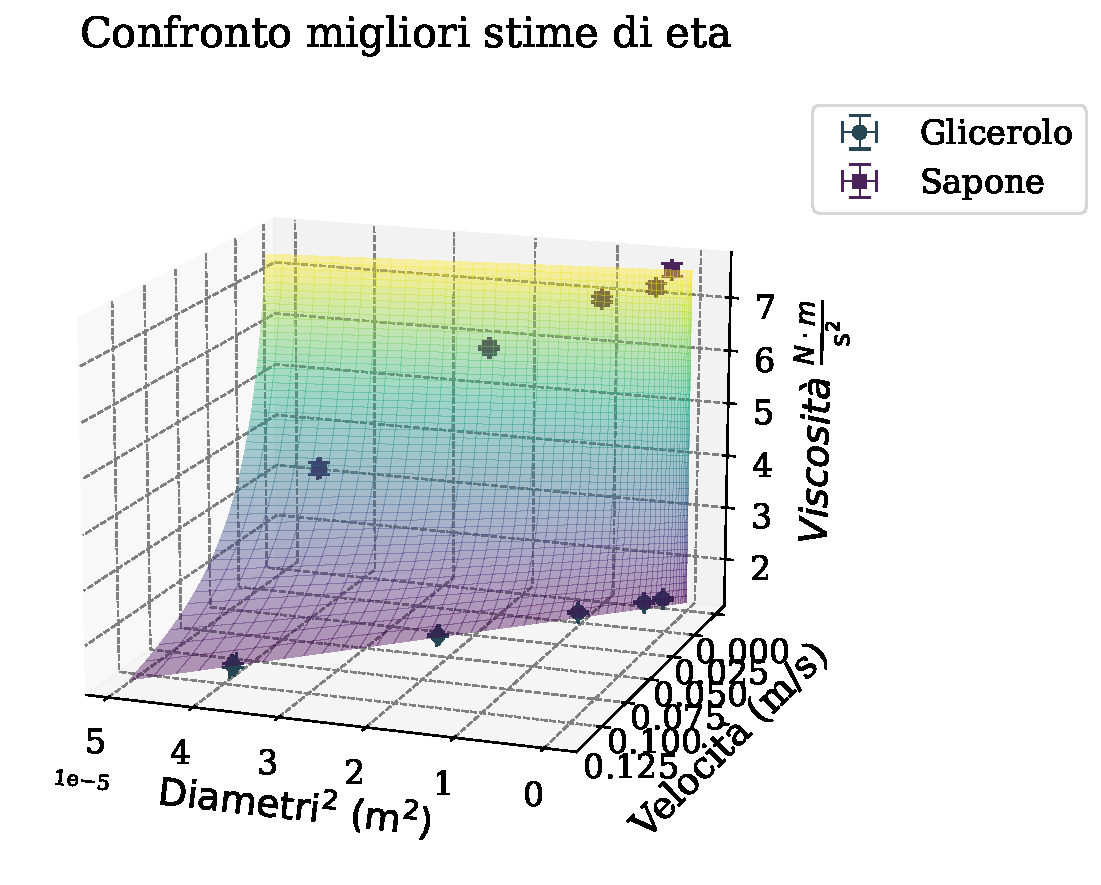
\includegraphics[width=0.52\textwidth]{confronto.pdf} 
    \caption    {Questo grafico rappresenta un confronto tridimensionale tra le misure della viscosità per glicerolo e sapone, qui la distinzione fra i due è evidente: il glicerolo (riga in basso) è lineare, mentre per il liquido saponoso la viscosità tende ad aumentare. (Questo è un grafico riassuntivo, non è stato utilizzato per svolgere test statistici) }  
    \label{Fig:1}  
    \end{figure}
In conclusione possiamo affermare che la legge di Stokes è stata verificata per il glicerolo nonostante le innumerevoli sistematiche che hanno intaccato l'accuratezza dei dati raccolti. Invece per quanto riguarda il liquido saponoso sono state riscontrate delle irregolarità, principalmente negli istogrammi (Fig.2, 3, e 4) e nel grafico che confronta diametri e viscosità (Fig.10), anche se rapportandolo alle incertezze, nettamente maggiori rispetto al glicerolo, in altri grafici come Fig.15 e 18 mostra un andamento simile a quello di un liquido newtoniano. Sul liquido saponoso ci si sarebbe aspettato di registrare un effetto memoria maggiore, ma probabilmente sarebbe stato possibile registrarlo se le misure fossero state prese al contrario: a partire dalle sferette di diametro maggiore a quelle di diametro minore. \\Per migliorare la stima della viscosità si sarebbe potuto innanzitutto aumentare il numero delle misurazioni; riuscire a stimare meglio la variazione di temperatura registrando la variazione di volume del liquido e verificando la percentuale di acqua contenuta nel glicerolo, o ancora meglio sarebbe stato mantenere la stanza a una temperatura statica per evitare fluttuazioni, e automatizzare il processo di raccolta dati per evitare l'errore umano dell'osservatore.   


\section{Appendice}


\subsection{Formulario}
\begin{enumerate}
    \item \textbf{Media pesata}
    \[
    \bar{x} = \frac{\sum_{i=1}^{n} \left(\frac{x_i}{w_i}\right)^2}{\sum_{i=1}^{n}\left(\frac{1}{w_i}\right)^2}
    \]
    
    \item \textbf{Incertezza sulla media pesata}
    \[
    \sigma_{\bar{x}} = \sqrt{\sum_{i=1}^{n}\left(\frac{1}{w_i}\right)^2}
    \]

    \item \textbf{Incertezza di una misurazione analogica}
    \[
    \sigma = \frac{R}{\sqrt{24}}
    \]
    dove \( R \) è la risoluzione strumentale.

    \item \textbf{Test di Student}
    \[
    t = \frac{x - x^*}{s_x}
    \]

    \item \textbf{Deviazione residua}
    \[
    \sigma = \sqrt{\frac{\sum \left( y_i - (a + bx_i) \right)^2}{N-2}}
    \]

    \item \textbf{Deviazione standard campionaria}
    \[
    s = \sqrt{\frac{1}{n-1} \sum_{i=1}^{n} \left(x_i - \bar{x}\right)^2}
    \]

    \item \textbf{Metodo \(\chi^2\)}
    \[
    \chi^2 = \sum_{i=1}^{N} \left(\frac{y_i - y_i^*}{s_{y_i}}\right)^2
    \]
    Dove \( y_i^* \) è il valore di \( y_i \) ottenuto dall'interpolazione e \( s_{y_i} \) è l'incertezza associata a \( y_i \).

    \item \textbf{Incertezza uniforme}
    \[
    \sigma = \frac{R}{\sqrt{12}}
    \]
    Dove \( R \) è la risoluzione strumentale.

    \item \textbf{Link al calcolatore del p-value}
    
    \text{Link:} \quad \url{http://courses.atlas.illinois.edu/spring2016/STAT/STAT200/pchisq.html}


    \item \textbf{Formula della propagazione delle incertezze nella correzione fondo parete}
    \[
    \sigma V_{\infty} = V_{\infty} \sqrt{\left( \frac{\partial V_l}{V_l} \right)^2 + \left( \frac{\partial \alpha}{\alpha} \right)^2 + \left( \frac{\partial \beta}{\beta} \right)^2}
    \]
    Dove
    \[
    \alpha = 1 + 2.33 \frac{r_i}{R} \quad \text{e} \quad \beta = 1 + 3.3 \frac{r_i}{h}
    \]

    \item \textbf{Errore relativo percentuale}
    \[
    \sigma_{\%} = \frac{\sigma x}{x} \times 100
    \]

\end{enumerate}


\subsection{Dati Sperimentali}
\small

\paragraph{Glicerolo}

\textbf{1.5 mm}
\begin{tabbing}
0.05 \quad \= 45.989 \quad \= 44.723 \quad \= 44.303 \quad \= 43.405 \kill % impostazione della larghezza
0.05 \> 45.989 \> 44.723 \> 44.303 \> 43.405 \\
0.10 \> 92.587 \> 90.079 \> 88.914 \> 87.401 \\
0.15 \> 140.058 \> 135.541 \> 133.313 \> 131.455 \\
0.20 \> 185.200 \> 181.375 \> 178.756 \> 175.651 \\
0.25 \> 231.558 \> 226.697 \> 223.498 \> 219.926 \\
0.30 \> 277.859 \> 272.304 \> 268.300 \> 263.920 \\
0.35 \> 324.024 \> 317.608 \> 313.124 \> 307.876 \\
0.40 \> 371.425 \> 363.377 \> 357.675 \> 352.055 \\
0.45 \> 416.571 \> 408.467 \> 402.542 \> 396.216 \\
0.50 \> 462.748 \> 454.368 \> 447.370 \> 441.500
\end{tabbing}

\textbf{2.5 mm}
\begin{tabbing}
0.05 \= 23.988 \quad \= 24.067 \quad \= 23.583 \quad \= 23.621 \kill
0.05 \> 23.988 \> 24.067 \> 23.583 \> 23.621 \\
0.10 \> 48.737 \> 48.281 \> 47.893 \> 47.440 \\
0.15 \> 73.272 \> 72.775 \> 72.117 \> 71.306 \\
0.20 \> 98.086 \> 96.970 \> 96.059 \> 95.492 \\
0.25 \> 122.536 \> 121.371 \> 120.528 \> 119.326 \\
0.30 \> 146.885 \> 145.739 \> 144.476 \> 143.383 \\
0.35 \> 171.885 \> 170.347 \> 168.268 \> 167.565 \\
0.40 \> 196.468 \> 194.734 \> 192.684 \> 191.778 \\
0.45 \> 221.356 \> 219.425 \> 217.221 \> 215.861 \\
0.50 \> 246.683 \> 243.585 \> 241.547 \> 239.927
\end{tabbing}

\textbf{4/32''}
\begin{tabbing}
0.05 \= 8.070 \quad \= 8.941 \quad \= 8.915 \quad \= 8.996 \kill
0.05 \> 8.070 \> 8.941 \> 8.915 \> 8.996 \\
0.10 \> 17.332 \> 18.219 \> 17.933 \> 18.133 \\
0.15 \> 26.596 \> 27.299 \> 27.122 \> 27.218 \\
0.20 \> 35.932 \> 36.700 \> 36.448 \> 36.379 \\
0.25 \> 45.279 \> 46.036 \> 45.670 \> 35.759 \\
0.30 \> 54.765 \> 55.296 \> 56.090 \> 54.888 \\
0.35 \> 63.952 \> 64.595 \> 64.017 \> 64.066 \\
0.40 \> 73.196 \> 73.861 \> 73.330 \> 73.850 \\
0.45 \> 82.639 \> 83.326 \> 82.624 \> 82.751 \\
0.50 \> 92.061 \> 92.532 \> 91.983 \> 91.595
\end{tabbing}

\textbf{6/32''}
\begin{tabbing}
0.05 \= 3.165 \quad \= 3.366 \quad \= 3.554 \quad \= 3.463 \kill
0.05 \> 3.165 \> 3.366 \> 3.554 \> 3.463 \\
0.10 \> 6.765 \> 6.759 \> 7.129 \> 6.960 \\
0.15 \> 10.374 \> 10.411 \> 10.601 \> 10.373 \\
0.20 \> 13.999 \> 13.933 \> 13.882 \> 13.833 \\
0.25 \> 17.417 \> 17.223 \> 17.700 \> 17.522 \\
0.30 \> 21.096 \> 21.063 \> 21.152 \> 21.134 \\
0.35 \> 24.751 \> 24.628 \> 24.668 \> 24.588 \\
0.40 \> 27.975 \> 28.247 \> 28.346 \> 28.086 \\
0.45 \> 31.802 \> 31.831 \> 31.832 \> 31.665 \\
0.50 \> 35.459 \> 35.271 \> 35.503 \> 35.191
\end{tabbing}

\textbf{8/32''}
\begin{tabbing}
0.10 \= 1.595 \quad \= 1.957 \quad \= 1.812 \quad \= 1.598 \kill
0.10 \> 1.595 \> 1.957 \> 1.812 \> 1.598 \\
0.20 \> 4.320 \> 4.306 \> 4.313 \> 4.094 \\
0.30 \> 6.960 \> 6.315 \> 6.850 \> 6.627 \\
0.40 \> 9.650 \> 9.074 \> 9.340 \> 9.124 \\
0.50 \> 12.475 \> 11.716 \> 12.087 \> 11.703
\end{tabbing}

\paragraph{Sapone}

\textbf{1.5 mm}
\begin{tabbing}
0.05 \= 45.989 \quad \= 44.723 \quad \= 44.303 \quad \= 43.405 \kill
0.05 \> 45.989 \> 44.723 \> 44.303 \> 43.405 \\
0.10 \> 92.587 \> 90.079 \> 88.914 \> 87.401 \\
0.15 \> 140.058 \> 135.541 \> 133.313 \> 131.455 \\
0.20 \> 185.200 \> 181.375 \> 178.756 \> 175.651 \\
0.25 \> 231.558 \> 226.697 \> 223.498 \> 219.926 \\
0.30 \> 277.859 \> 272.304 \> 268.300 \> 263.920 \\
0.35 \> 324.024 \> 317.608 \> 313.124 \> 307.876 \\
0.40 \> 371.425 \> 363.377 \> 357.675 \> 352.055 \\
0.45 \> 416.571 \> 408.467 \> 402.542 \> 396.216 \\
0.50 \> 462.748 \> 454.368 \> 447.370 \> 441.500
\end{tabbing}

\textbf{2.5 mm}
\begin{tabbing}
0.05 \= 23.988 \quad \= 24.067 \quad \= 23.583 \quad \= 23.621 \kill
0.05 \> 23.988 \> 24.067 \> 23.583 \> 23.621 \\
0.10 \> 48.737 \> 48.281 \> 47.893 \> 47.440 \\
0.15 \> 73.272 \> 72.775 \> 72.117 \> 71.306 \\
0.20 \> 98.086 \> 96.970 \> 96.059 \> 95.492 \\
0.25 \> 122.536 \> 121.371 \> 120.528 \> 119.326 \\
0.30 \> 146.885 \> 145.739 \> 144.476 \> 143.383 \\
0.35 \> 171.885 \> 170.347 \> 168.268 \> 167.565 \\
0.40 \> 196.468 \> 194.734 \> 192.684 \> 191.778 \\
0.45 \> 221.356 \> 219.425 \> 217.221 \> 215.861 \\
0.50 \> 246.683 \> 243.585 \> 241.547 \> 239.927
\end{tabbing}

\textbf{4/32''}
\begin{tabbing}
0.05 \= 8.070 \quad \= 8.941 \quad \= 8.915 \quad \= 8.996 \kill
0.05 \> 8.070 \> 8.941 \> 8.915 \> 8.996 \\
0.10 \> 17.332 \> 18.219 \> 17.933 \> 18.133 \\
0.15 \> 26.596 \> 27.299 \> 27.122 \> 27.218 \\
0.20 \> 35.932 \> 36.700 \> 36.448 \> 36.379 \\
0.25 \> 45.279 \> 46.036 \> 45.670 \> 35.759 \\
0.30 \> 54.765 \> 55.296 \> 56.090 \> 54.888 \\
0.35 \> 63.952 \> 64.595 \> 64.017 \> 64.066 \\
0.40 \> 73.196 \> 73.861 \> 73.330 \> 73.850 \\
0.45 \> 82.639 \> 83.326 \> 82.624 \> 82.751 \\
0.50 \> 92.061 \> 92.532 \> 91.983 \> 91.595
\end{tabbing}

\textbf{6/32''}
\begin{tabbing}
0.05 \= 3.165 \quad \= 3.366 \quad \= 3.554 \quad \= 3.463 \kill
0.05 \> 3.165 \> 3.366 \> 3.554 \> 3.463 \\
0.10 \> 6.765 \> 6.759 \> 7.129 \> 6.960 \\
0.15 \> 10.374 \> 10.411 \> 10.601 \> 10.373 \\
0.20 \> 13.999 \> 13.933 \> 13.882 \> 13.833 \\
0.25 \> 17.417 \> 17.223 \> 17.700 \> 17.522 \\
0.30 \> 21.096 \> 21.063 \> 21.152 \> 21.134 \\
0.35 \> 24.751 \> 24.628 \> 24.668 \> 24.588 \\
0.40 \> 27.975 \> 28.247 \> 28.346 \> 28.086 \\
0.45 \> 31.802 \> 31.831 \> 31.832 \> 31.665 \\
0.50 \> 35.459 \> 35.271 \> 35.503 \> 35.191
\end{tabbing}

\textbf{8/32''}
\begin{tabbing}
0.10 \= 1.595 \quad \= 1.957 \quad \= 1.812 \quad \= 1.598 \kill
0.10 \> 1.595 \> 1.957 \> 1.812 \> 1.598 \\
0.20 \> 4.320 \> 4.306 \> 4.313 \> 4.094 \\
0.30 \> 6.960 \> 6.315 \> 6.850 \> 6.627 \\
0.40 \> 9.650 \> 9.074 \> 9.340 \> 9.124 \\
0.50 \> 12.475 \> 11.716 \> 12.087 \> 11.703
\end{tabbing}

\subsection{Elaborati Completi}
Vengono riportati, in questo ordine, gli elaborati completi delle figure 13, 14, 17 e 18.
%\paragraph{Figura 13}
\includepdf[pages=-]{gli_elaborato_profondita.pdf}
%\paragraph{Figura 14}
\includepdf[pages=-]{sap_elaborato_profondita.pdf}
%\paragraph{Figura 17}
\includepdf[pages=-]{gli_elaborato_memoria.pdf}
%\paragraph{Figura 18}
\includepdf[pages=-]{sap_elaborato_memoria.pdf}

\end{multicols}
\end{document}
